\documentclass[border=2pt]{standalone}
\usepackage{tikz}
\usetikzlibrary{arrows.meta,chains}

\begin{document}
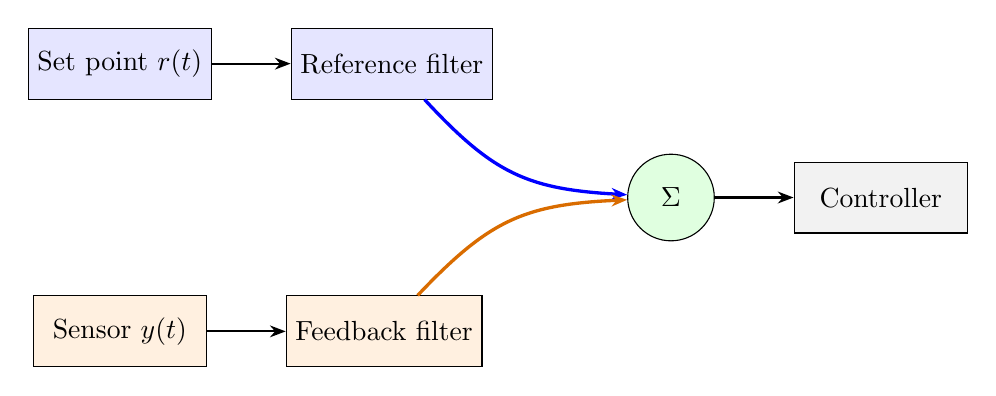
\begin{tikzpicture}[
  start chain=reference going right,
  start chain=feedback going right,
  start chain=control going right,
  block/.style={draw,minimum width=22mm,minimum height=9mm,align=center},
  every join/.style={-{Stealth[length=2mm]},very thick}
]
  \node[block,on chain=reference,fill=blue!10] (setpoint) at (0,1.7) {Set point $r(t)$};
  \node[block,on chain=reference,fill=blue!10] (reference-filter) {Reference filter};

  \node[block,on chain=feedback,fill=orange!12] (sensor) at (0,-1.7) {Sensor $y(t)$};
  \node[block,on chain=feedback,fill=orange!12] (feedback-filter) {Feedback filter};

  \node[
    draw,
    circle,
    minimum size=11mm,
    on chain=control,
    fill=green!12,
    join=with reference-end by {blue,bend right=22,looseness=1.15},
    join=with feedback-end by {orange!85!black,bend left=22,looseness=1.15}
  ] (sum) at (7,0) {$\Sigma$};

  \node[
    block,
    on chain=control,
    fill=gray!10,
    join=by {black,out=0,in=180,looseness=1.05}
  ] (controller) {Controller};

  \path[-{Stealth[length=2mm]},thick]
    (setpoint) edge (reference-filter)
    (sensor) edge (feedback-filter);
\end{tikzpicture}
\end{document}
